%%%%%%%%%%%%%%%%%%%%%%%%%%%%%%%%%%%%%%%%%
% University/School Laboratory Report
% LaTeX Template
% Version 4.0 (March 21, 2022)
%
% This template originates from:
% https://www.LaTeXTemplates.com
%
% Authors:
% Vel (vel@latextemplates.com)
% Linux and Unix Users Group at Virginia Tech Wiki
%
% License:
% CC BY-NC-SA 4.0 (https://creativecommons.org/licenses/by-nc-sa/4.0/)
%
%%%%%%%%%%%%%%%%%%%%%%%%%%%%%%%%%%%%%%%%%

%----------------------------------------------------------------------------------------
%	PACKAGES AND DOCUMENT CONFIGURATIONS
%----------------------------------------------------------------------------------------

\documentclass[
	letterpaper, % Paper size, specify a4paper (A4) or letterpaper (US letter)
	10pt, % Default font size, specify 10pt, 11pt or 12pt
]{CSUniSchoolLabReport}

%----------------------------------------------------------------------------------------
%	REPORT INFORMATION
%----------------------------------------------------------------------------------------

\title{ECE 398-MA \\ Introduction to Modern Communication with Python and SDR \\ Python Lab 3} % Report title

\author{Noah Breit} % Author name(s), add additional authors like: '\& James \textsc{Smith}'

\date{\today} % Date of the report

%----------------------------------------------------------------------------------------

\begin{document}

\maketitle % Insert the title, author and date using the information specified above

% \begin{center}
% 	\begin{tabular}{l r}
% 		Date Performed: & February 13, 2022 \\ % Date the experiment was performed
% 		Partners: & Cecilia \textsc{Smith} \\ % Partner names
% 		& Tajel \textsc{Khumalo} \\
% 		Instructor: & Professor \textsc{Rivera} % Instructor/supervisor
% 	\end{tabular}
% \end{center}

% If you need to include an abstract, uncomment the lines below
%\begin{abstract}
%	Abstract text
%\end{abstract}

%----------------------------------------------------------------------------------------
%	OBJECTIVE
%----------------------------------------------------------------------------------------

\section{Assignment 1}

\begin{lstlisting}[language=Python]
	
	import numpy as np
	import matplotlib.pyplot as plt
	
	# Define simulation parameters
	N = 1000    # Number of samples
	fs = 100e3  # Sampling rate (Hz)
	dt = 1/fs   # Sampling period
	fc = 20e3   # Carrier frequency (Hz)
	t = np.arange(N) / fs  # Time vector
	
	# FM/PM Modulation Parameters
	kf = 500  # Frequency deviation constant (for FM)
	kp = np.pi / 2  # Phase deviation constant (for PM)
	
	# Original Message Signal (square wave)
	original_message = np.concatenate([np.ones(N//2), -1*np.ones(N//2)])
	
	# Modified Message Signal (integral of the original square wave)
	modified_message = np.cumsum(original_message) * dt
	
	# FM Modulation (integrate original message signal)
	integrated_message = np.cumsum(original_message) * dt
	fm_signal = np.cos(2 * np.pi * fc * t + 2 * np.pi * kf * integrated_message)
	
	# PM Modulation (use modified message signal)
	pm_signal = np.cos(2 * np.pi * fc * t + kp * modified_message)
	
	# Plot results
	plt.figure()
	plt.subplot(3, 1, 1)
	plt.plot(t, modified_message, label='Modified Message')
	plt.xlabel("Time [s]")
	plt.ylabel("Amplitude")
	plt.legend()
	
	plt.subplot(3, 1, 2)
	plt.plot(t, fm_signal, label='FM')
	plt.xlabel("Time [s]")
	plt.ylabel("Amplitude")
	plt.legend()
	
	plt.subplot(3, 1, 3)
	plt.plot(t, pm_signal, label='PM')
	plt.xlabel("Time [s]")
	plt.ylabel("Amplitude")
	plt.legend()
	plt.tight_layout()
	plt.savefig('assignment1b.png')
	plt.show()

\end{lstlisting}

\begin{figure}[H] % [H] forces the figure to be placed exactly where it appears in the text
	\centering % Horizontally center the figure
	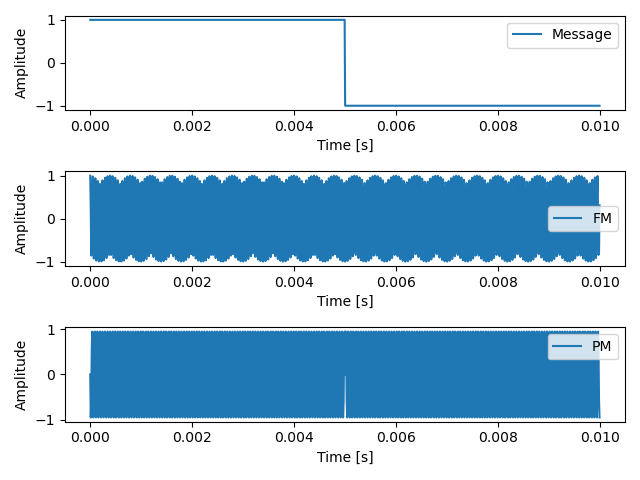
\includegraphics[width=1.2\textwidth]{assignment1a.png} % Include the figure
	\caption{Original FM and PM Signals}
	\label{fig:block}
\end{figure}

\begin{figure}[H] % [H] forces the figure to be placed exactly where it appears in the text
	\centering % Horizontally center the figure
	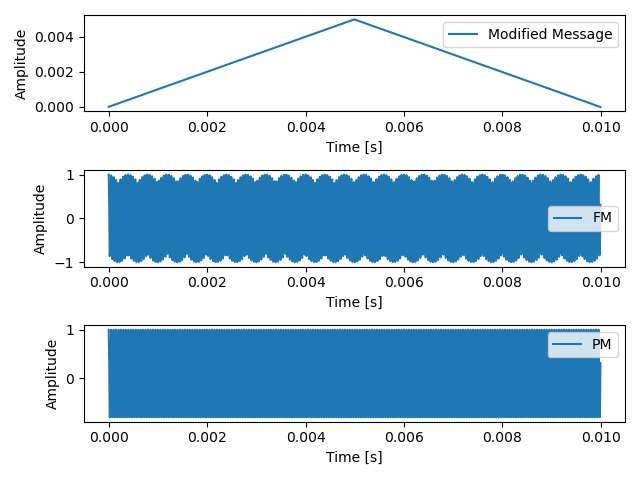
\includegraphics[width=1.2\textwidth]{assignment1b.png} % Include the figure
	\caption{Modified FM and PM Signals}
	\label{fig:block}
\end{figure}

\section{Assignment 2}

\begin{lstlisting}[language=Python]
	
	# Define simulation parameters
	N = 1000    # Number of samples
	fs = 100e3  # Sampling rate (Hz)
	dt = 1/fs   # Sampling period
	fc = 20e3    # Carrier frequency (Hz)
	t = np.arange(N) / fs  # Time vector
	
	# FM/PM Modulation Parameters
	kf = 500  # Frequency deviation constant (for FM)
	kp = np.pi / 2  # Phase deviation constant (for PM)
	
	# Reuse/modify the code in Part 1
	
	fc = 20e3    # Carrier frequency (Hz)
	
	
	# Message signal (single-tone sinusoid)
	fm = 1000 # message frequency
	message = np.sin(2*np.pi*fm/fs*np.arange(N))
	
	# Define FM/PM Modulation Parameters
	kf_narrow = 10  # narrowband FM deviation 
	kf_wide = 500  # wideband  deviation 
	kp = np.pi / 2  # PM deviation 
	
	# Compute the effective bandwidth
	B_fm_narrow = 2 * (kf_narrow * max(abs(message)) + fm)
	B_fm_wide = 2 * (kf_wide * max(abs(message)) + fm)
	B_pm = 2 * (kp * max(abs(message)) + 1) * fm
	
	print('B_fm_narrow (Hz): ', B_fm_narrow)
	print('B_fm_wide (Hz): ', B_fm_wide)
	print('B_pm (Hz): ', B_pm)
	
	# Plot the spectrum of narrowband FM, wideband FM, and PM
	# Plot spectrum in linear scale
	def plot_spectrum(signal, title):
	spectrum = np.fft.fft(signal)
	freq = np.fft.fftfreq(N, dt)
	plt.plot(freq[:N // 2], abs(spectrum[:N // 2]))
	plt.title(title)
	plt.xlabel("Frequency [Hz]")
	plt.ylabel("Amplitude")
	plt.grid()
	
	# Generate narrowband FM signal
	integrated_message = np.cumsum(message) * dt
	fm_signal_narrow = np.cos(2 * np.pi * fc * np.arange(N) / fs + 2 * np.pi * kf_narrow * integrated_message)
	
	# Generate wideband FM signal
	fm_signal_wide = np.cos(2 * np.pi * fc * np.arange(N) / fs + 2 * np.pi * kf_wide * integrated_message)
	
	# Generate PM signal
	pm_signal = np.cos(2 * np.pi * fc * np.arange(N) / fs + kp * message)
	
	# Spectrum of narrowband FM signal
	plt.figure()
	plt.subplot(3, 1, 1)
	plot_spectrum(fm_signal_narrow, "Spectrum of Narrowband FM")
	
	# Spectrum of wideband FM signal
	plt.subplot(3, 1, 2)
	plot_spectrum(fm_signal_wide, "Spectrum of Wideband FM")
	
	# Spectrum of PM signal
	plt.subplot(3, 1, 3)
	plot_spectrum(pm_signal, "Spectrum of PM")
	
	plt.tight_layout()
	plt.savefig('assignment2.png')
	plt.show()

\end{lstlisting}

\begin{figure}[H] % [H] forces the figure to be placed exactly where it appears in the text
	\centering % Horizontally center the figure
	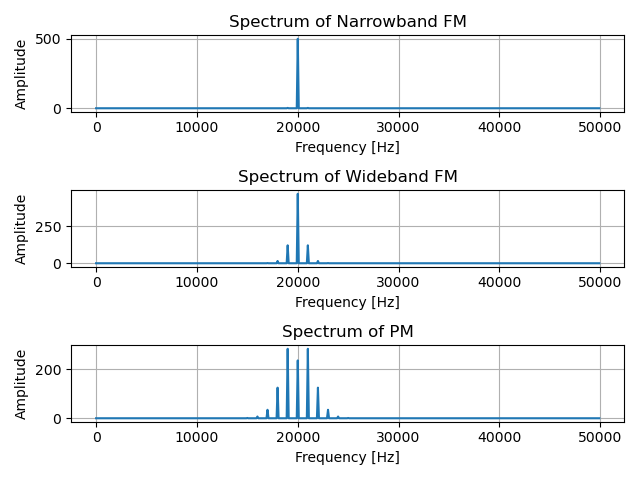
\includegraphics[width=1.2\textwidth]{assignment2.png} % Include the figure
	\caption{FM and PM Spectrum}
	\label{fig:block}
\end{figure}

Serial output: 					\newline
B-fm-narrow (Hz):  2020.0 		\newline
B-fm-wide (Hz):  3000.0			\newline
B-pm (Hz):  5141.592653589793	\newline

Visually, the graph outputs had the following bandwidths:	\newline
B-fm-narrow (Hz):  ~1000.0		\newline
B-fm-wide (Hz):  ~2500.0		\newline
B-pm (Hz):  ~5000.0				\newline

These numbers are within margin of error due to the scale of the graphs. So the calculations were correct.

\section{Assignment 3}

\begin{lstlisting}[language=Python]
	# Reuse the code for FM/PM modulation from Part 2
	
	# Define FM demodulation function
	def fmdemod(x, fc, fs, kf):
	"""
	Demodulate FM using the Hilbert transform.
	
	Parameters:
	x: ndarray
	Received FM signal
	fc: float
	Carrier frequency (Hz)
	fs: float
	Sampling rate (Hz)
	kf: float
	Frequency deviation constant
	
	Returns:
	m: ndarray
	Recovered message signal
	"""
	# Apply Hilbert transform to get the analytic signal
	z = hilbert(x)
	# Extract the instantaneous phase
	inst_phase = np.unwrap(np.angle(z))
	# Calculate the instantaneous frequency deviation
	# np.diff() ~> derivative
	inst_freq = np.diff(inst_phase) * fs / (2.0 * np.pi) 
	# Subtract carrier frequency and scale by kf to recover message signal
	m = (inst_freq - fc) / kf
	# Match length of output with input by appending last value
	return np.concatenate((m, [m[-1]]))
	
	# Define PM demodulation function
	def pmdemod(x, fc, fs, kp):
	"""
	Demodulate PM using the Hilbert transform.
	
	Parameters:
	x: ndarray
	Received PM signal
	fc: float
	Carrier frequency (Hz)
	fs: float
	Sampling rate (Hz)
	kp: float
	Phase deviation constant
	
	Returns:
	m: ndarray
	Recovered message signal
	"""
	# Apply Hilbert transform to get the analytic signal
	z = hilbert(x)
	# Extract the instantaneous phase
	inst_phase = np.unwrap(np.angle(z))
	# Subtract carrier phase term to isolate modulated phase component
	carrier_phase = 2 * np.pi * fc * np.arange(len(x)) / fs
	m = (inst_phase - carrier_phase) / kp  # Scale by phase deviation constant
	return m
	
	# Reuse simulation parameters from Part 2
	N = 1000  # Number of samples
	fs = 100e3  # Sampling rate (Hz)
	dt = 1/fs  # Sampling period
	fc = 20e3  # Carrier frequency (Hz)
	t = np.arange(N) / fs  # Time vector
	
	kf_narrow = 10  # Narrowband FM deviation constant
	kf_wide = 500   # Wideband FM deviation constant
	kp = np.pi / 2  # PM deviation constant
	
	# Message signal (single-tone sinusoid)
	fm = 1000  # Message frequency (Hz)
	message = np.sin(2 * np.pi * fm * t)
	
	# Generate modulated signals from Part 2 code:
	integrated_message = np.cumsum(message) * dt
	
	fm_signal_narrow = np.cos(2 * np.pi * fc * t + 2 * np.pi * kf_narrow * integrated_message)
	fm_signal_wide = np.cos(2 * np.pi * fc * t + 2 * np.pi * kf_wide * integrated_message)
	pm_signal = np.cos(2 * np.pi * fc * t + kp * message)
	
	# Demodulate FM and PM signals using implemented functions
	fm_narrow_demod = fmdemod(fm_signal_narrow, fc, fs, kf_narrow)
	fm_wide_demod = fmdemod(fm_signal_wide, fc, fs, kf_wide)
	pm_demod = pmdemod(pm_signal, fc, fs, kp)
	
	# Plot results for comparison with original message signal
	plt.figure()
	plt.subplot(4, 1, 1)
	plt.plot(t, message, label='Message')
	plt.legend()
	plt.subplot(4, 1, 2)
	plt.plot(t, fm_narrow_demod, label='FM Narrowband Demodulated')
	plt.legend()
	plt.subplot(4, 1, 3)
	plt.plot(t, fm_wide_demod, label='FM Wideband Demodulated')
	plt.legend()
	plt.subplot(4, 1, 4)
	plt.plot(t, pm_demod, label='PM Demodulated')
	plt.legend()
	plt.tight_layout()
	plt.savefig("assignment3.png")
	plt.show()

\end{lstlisting}

\begin{figure}[H] % [H] forces the figure to be placed exactly where it appears in the text
	\centering % Horizontally center the figure
	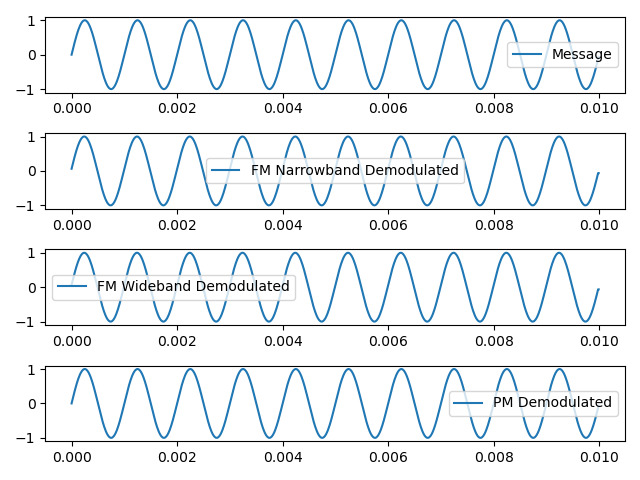
\includegraphics[width=1.2\textwidth]{assignment3.png} % Include the figure
	\caption{Original Signal + FM-Narrow-Band, FM-Wide-Band, and PM Demodulated Signals}
	\label{fig:block}
\end{figure}

\end{document}